\documentclass[aspectratio=169]{beamer}
\usepackage{booktabs}
\usepackage{colortbl}
\usepackage{array}
\usepackage{xcolor}
\usepackage{tikz}
\usepackage{amsmath}

% ── Color Palette ─────────────────────────────────────────────────────────────
\definecolor{navy}{HTML}{0D1B2A}
\definecolor{navymid}{HTML}{1B2E45}
\definecolor{teal}{HTML}{0D9488}
\definecolor{teallt}{HTML}{5EEAD4}
\definecolor{offwhite}{HTML}{F0F4F8}
\definecolor{graylt}{HTML}{E2E8F0}
\definecolor{mygray}{HTML}{94A3B8}
\definecolor{amber}{HTML}{F59E0B}
\definecolor{mygreen}{HTML}{22C55E}
\definecolor{mytext}{HTML}{1E293B}
\definecolor{lightyellow}{HTML}{FFF3CD}
\definecolor{lightgreen}{HTML}{E8F5E9}

% ── Beamer Theme ──────────────────────────────────────────────────────────────
\usetheme{default}
\usecolortheme[named=navy]{structure}
\setbeamercolor{normal text}{fg=mytext, bg=offwhite}
\setbeamercolor{frametitle}{fg=white, bg=navy}
\setbeamertemplate{navigation symbols}{}
\setbeamertemplate{footline}{}
\setbeamerfont{frametitle}{size=\large, series=\bfseries}

\setbeamertemplate{frametitle}{%
  \nointerlineskip
  \begin{beamercolorbox}[wd=\paperwidth, ht=0.6cm, dp=0.15cm]{frametitle}
    
\begin{tikzpicture}[overlay]
      \fill[teal] (0,0) rectangle (0.12,0.75);
    \end{tikzpicture}
    \hspace{0.25cm}\insertframetitle
  \end{beamercolorbox}
}

\newcommand{\sectionbar}{%
  {\color{teal}\rule{\linewidth}{0.4pt}}\\[2pt]}

% ── Document ──────────────────────────────────────────────────────────────────
\begin{document}

% ─── SLIDE 1: Title ───────────────────────────────────────────────────────────
\begin{frame}[plain]
  \begin{tikzpicture}[remember picture, overlay]
    \fill[navy] (current page.south west) rectangle (current page.north east);
    \fill[teal] (current page.south west)
      rectangle ([xshift=0.18cm] current page.north west);
  \end{tikzpicture}
  \vspace{1.2cm}
  {\color{white}\LARGE\bfseries Weapon-Target Assignment}\\[0.4cm]
  {\color{teallt}\large 03. Explanation of  MMR \& Genetic Algorithm}\\[0.3cm]
  {\color{teal}\rule{7cm}{0.4pt}}\\[0.4cm]
  {\color{mygray}\itshape Step-by-step illustration with a $3\times3$ instance}
  \vspace{1.0cm}

  
\begin{tikzpicture}
    \foreach \lbl [count=\i] in {3 Weapons, 3 Targets, Known Kill Probs}{
      \node[draw=teal, fill=navymid, text=teallt, rounded corners=3pt,
            inner sep=5pt, font=\small] at (\i*3.5cm-1.75cm, 0) {\lbl};
    }
  \end{tikzpicture}
\end{frame}

% ─── SLIDE 2: Problem Instance ────────────────────────────────────────────────
\begin{frame}{Problem Instance}
  \begin{columns}[T]
    \begin{column}{0.57\textwidth}
      {\small\bfseries\color{navy} Target Values}\\[4pt]
      \begin{tabular}{>{\columncolor{teal}\color{white}\bfseries}l
                      >{\columncolor{lightgreen}}c
                      >{\columncolor{lightgreen}}c
                      >{\columncolor{lightgreen}}c}
        \toprule
        \rowcolor{navy}
          \color{white} &
          \color{white}Target 0 &
          \color{white}Target 1 &
          \color{white}Target 2 \\
        \midrule
        Value & 10 & 20 & 30 \\
        \bottomrule
      \end{tabular}

      \vspace{0.35cm}
      {\small\bfseries\color{navy}
        Kill Probabilities $p[\text{weapon}][\text{target}]$}\\[4pt]
      \begin{tabular}{>{\columncolor{teal}\color{white}\bfseries}l ccc}
        \toprule
        \rowcolor{navy}
          \color{white} &
          \color{white}Target 0 &
          \color{white}Target 1 &
          \color{white}Target 2 \\
        \midrule
        Weapon 0 & 0.3 & 0.2 & 0.1 \\
        Weapon 1 & 0.1 & 0.4 & 0.2 \\
        Weapon 2 & 0.2 & 0.3 &
          \cellcolor{lightyellow}\textbf{0.5} \\
        \bottomrule
      \end{tabular}
    \end{column}

    \begin{column}{0.38\textwidth}
      \colorbox{navy}{%
        \begin{minipage}{\linewidth}
          \vspace{0.2cm}\centering
          {\color{teal}\bfseries Objective}\\[0.2cm]
          {\color{white}\small Minimize total\\survival value\\of all targets}\\[0.25cm]
          {\color{teallt}\bfseries
            $\displaystyle\sum_j V_j \cdot \prod_i (1-p_{ij})$}\\[0.25cm]
          {\color{mygray}\small Each weapon assigned\\to exactly one target}
          \vspace{0.2cm}
        \end{minipage}}
    \end{column}
  \end{columns}

  \vspace{0.25cm}
  \colorbox{navymid}{\begin{minipage}{\linewidth}
    {\color{graylt}\small\itshape
     Both algorithms solve the same problem ---
     they differ in \emph{how} they search for the optimal allocation.}
  \end{minipage}}
\end{frame}

% ─── SLIDE 3a: MMR Description ────────────────────────────────────────────────
\begin{frame}{MMR Algorithm --- Overview}

  {\large\bfseries\color{navy} Maximum Marginal Return (Greedy)}\\[3pt]

  \begin{columns}[T]
    \begin{column}{0.65\textwidth}
      \begin{enumerate}\itemsep10pt
        \item \textbf{Scan all pairs}\\[2pt]
          {\small For every unallocated weapon $w$ and every target $t$:}\\[2pt]
          {\small\colorbox{navymid}{\color{teallt}
            $\;\text{decrease} = V[t] \times p[w][t]\;$}}

        \item \textbf{Pick best pair}\\[2pt]
          {\small Select weapon-target with \emph{maximum} decrease}\\
          {\small\color{mygray} ``most bang for the buck''}

        \item \textbf{Assign \& update}\\[2pt]
          {\small Assign weapon $\to$ target.\quad
            $V[t] \mathrel{-}= \text{maxDecrease}$}\\
          {\small Remove weapon from pool.}

        \item \textbf{Repeat}\\[2pt]
          {\small Return to step~1 until all weapons assigned.}
      \end{enumerate}
    \end{column}

    \begin{column}{0.40\textwidth}
      \colorbox{offwhite}{\begin{minipage}{\linewidth}
        \vspace{6pt}
        {\small\bfseries\color{teal} Key Properties}\\[6pt]
        {\small\color{navy}\bfseries Complexity:\;}
          {\small $O(W^2 \times T)$}\\[5pt]
        {\small\color{navy}\bfseries Deterministic:\;}
          {\small same input $\to$ same output}\\[5pt]
        {\small\color{navy}\bfseries Optimality:\;}
          {\small local optimum only}\\[5pt]
        {\small\color{navy}\bfseries Speed:\;}
          {\small very fast, single pass}
        \vspace{6pt}
      \end{minipage}}

      \vspace{10pt}
      \colorbox{navymid}{\begin{minipage}{\linewidth}
        \vspace{5pt}
        {\color{teallt}\small\itshape
         Greedy commits to the locally best choice each round ---
         fast but may miss the globally optimal solution.}
        \vspace{5pt}
      \end{minipage}}
    \end{column}
  \end{columns}
\end{frame}

% ─── SLIDE 3b: MMR Pseudocode ────────────────────────────────────────\begin{frame}{MMR Algorithm --- Pseudocode}

\begin{frame}{MMR Algorithm --- Pseudocode}
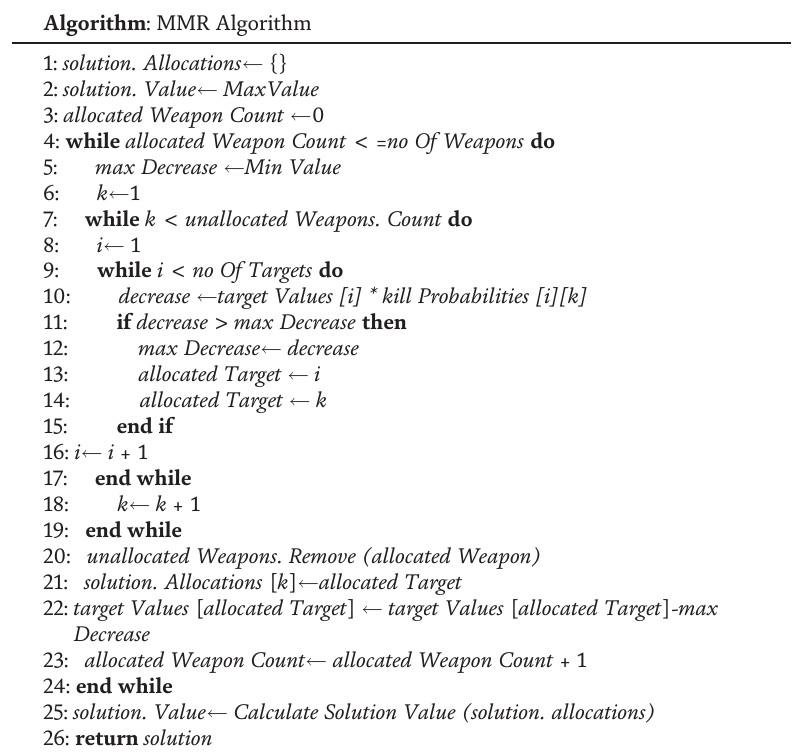
\includegraphics[width=\textwidth, height=0.85\textheight, keepaspectratio]{Screenshot 2026-03-29 153944.png}
\end{frame}
% ─── SLIDE 4: MMR Round 1 ─────────────────────────────────────────────────────
\begin{frame}{MMR --- Round 1: Find Maximum Decrease}
  {\small Scan all pairs.\quad
    $\text{decrease} = \text{current\_value}[t]
      \times \text{kill\_prob}[w][t]$}

  \begin{columns}[T]
    \begin{column}{0.57\textwidth}
      \vspace{4pt}
      \begin{tabular}{cccc}
        \toprule
        \rowcolor{navy}
          \color{white}\bfseries Weapon &
          \color{white}\bfseries Target &
          \color{white}\bfseries Calculation &
          \color{white}\bfseries Decrease \\
        \midrule
        W0 & T0 & $10\times0.3$ & 3.0 \\
        W0 & T1 & $20\times0.2$ & 4.0 \\
        W0 & T2 & $30\times0.1$ & 3.0 \\
        W1 & T0 & $10\times0.1$ & 1.0 \\
        W1 & T1 & $20\times0.4$ & 8.0 \\
        W1 & T2 & $30\times0.2$ & 6.0 \\
        W2 & T0 & $10\times0.2$ & 2.0 \\
        W2 & T1 & $20\times0.3$ & 6.0 \\
        \rowcolor{lightyellow}
        \bfseries W2 & \bfseries T2 &
          $\bfseries 30\times0.5$ &
          \cellcolor{amber}\color{white}\bfseries 15.0 $\leftarrow$ MAX \\
        \bottomrule
      \end{tabular}
    \end{column}

    \begin{column}{0.38\textwidth}
      \colorbox{navy}{\begin{minipage}{\linewidth}
        \vspace{0.2cm}\centering
        {\color{teal}\bfseries Result}\\[0.2cm]
        {\color{white}\Large\bfseries W2 $\rightarrow$ T2}\\[0.15cm]
        {\color{amber} Decrease: 15.0}\\[0.2cm]
        {\color{teal}\rule{3cm}{0.3pt}}\\[0.15cm]
        {\color{mygray}\small Update:}\\
        {\color{teallt}\small $V[\text{T2}] = 30 - 15 = 15$}\\[0.1cm]
        {\color{mygray}\small W2 removed from pool}\\[0.1cm]
        {\color{teallt}\small Remaining: W0, W1}
        \vspace{0.2cm}
      \end{minipage}}
    \end{column}
  \end{columns}
\end{frame}

% ─── SLIDE 5: MMR Rounds 2 & 3 ───────────────────────────────────────────────
\begin{frame}{MMR --- Rounds 2 \& 3 $\rightarrow$ Final Result}
  \begin{columns}[T]
    \begin{column}{0.46\textwidth}
      \colorbox{navymid}{\color{teallt}\bfseries\small
        Round 2 | W: W0,W1 | V: T0=10,T1=20,T2=15}
      \vspace{3pt}

      \begin{tabular}{ccc}
        \toprule
        \rowcolor{navy}
          \color{white}\bfseries W$\times$T &
          \color{white}\bfseries Calc &
          \color{white}\bfseries Dec \\
        \midrule
        W0$\to$T0 & $10\times0.3$ & 3.0 \\
        W0$\to$T1 & $20\times0.2$ & 4.0 \\
        W0$\to$T2 & $15\times0.1$ & 1.5 \\
        W1$\to$T0 & $10\times0.1$ & 1.0 \\
        \rowcolor{lightyellow}
        \bfseries W1$\to$T1 & $\bfseries20\times0.4$ &
          \cellcolor{amber}\color{white}\bfseries 8.0$\leftarrow$ \\
        W1$\to$T2 & $15\times0.2$ & 3.0 \\
        \bottomrule
      \end{tabular}

      \vspace{4pt}
      {\small\bfseries\color{navy} W1 $\to$ T1}
      {\small $\;V[\text{T1}]=20-8=12$}
    \end{column}

    \begin{column}{0.46\textwidth}
      \colorbox{navymid}{\color{teallt}\bfseries\small
        Round 3 | W: W0 | V: T0=10,T1=12,T2=15}
      \vspace{3pt}

      \begin{tabular}{ccc}
        \toprule
        \rowcolor{navy}
          \color{white}\bfseries W$\times$T &
          \color{white}\bfseries Calc &
          \color{white}\bfseries Dec \\
        \midrule
        \rowcolor{lightyellow}
        \bfseries W0$\to$T0 & $\bfseries10\times0.3$ &
          \cellcolor{amber}\color{white}\bfseries 3.0$\leftarrow$ \\
        W0$\to$T1 & $12\times0.2$ & 2.4 \\
        W0$\to$T2 & $15\times0.1$ & 1.5 \\
        \bottomrule
      \end{tabular}

      \vspace{4pt}
      {\small\bfseries\color{navy} W0 $\to$ T0}
    \end{column}
  \end{columns}

  \vspace{0.25cm}
  \colorbox{navy}{\begin{minipage}{\linewidth}
    \vspace{0.15cm}\centering
    {\color{teal}\bfseries Final MMR Allocation}\\[0.15cm]
    \begin{tabular}{ccc}
      \colorbox{navymid}{\color{white}\small W0$\to$T0\;(p=0.3)} &
      \colorbox{navymid}{\color{white}\small W1$\to$T1\;(p=0.4)} &
      \colorbox{navymid}{\color{white}\small W2$\to$T2\;(p=0.5)}
    \end{tabular}\\[0.15cm]
    {\color{amber}\bfseries allocation = [0,\; 1,\; 2]}
    \vspace{0.15cm}
  \end{minipage}}
\end{frame}

% ─── SLIDE 6a: GA Description ────────────────────────────────────────────────

\begin{frame}{Genetic Algorithm --- Overview}

  \begin{columns}[T]
    % Left column: figure
    \begin{column}{0.65\textwidth}
    
      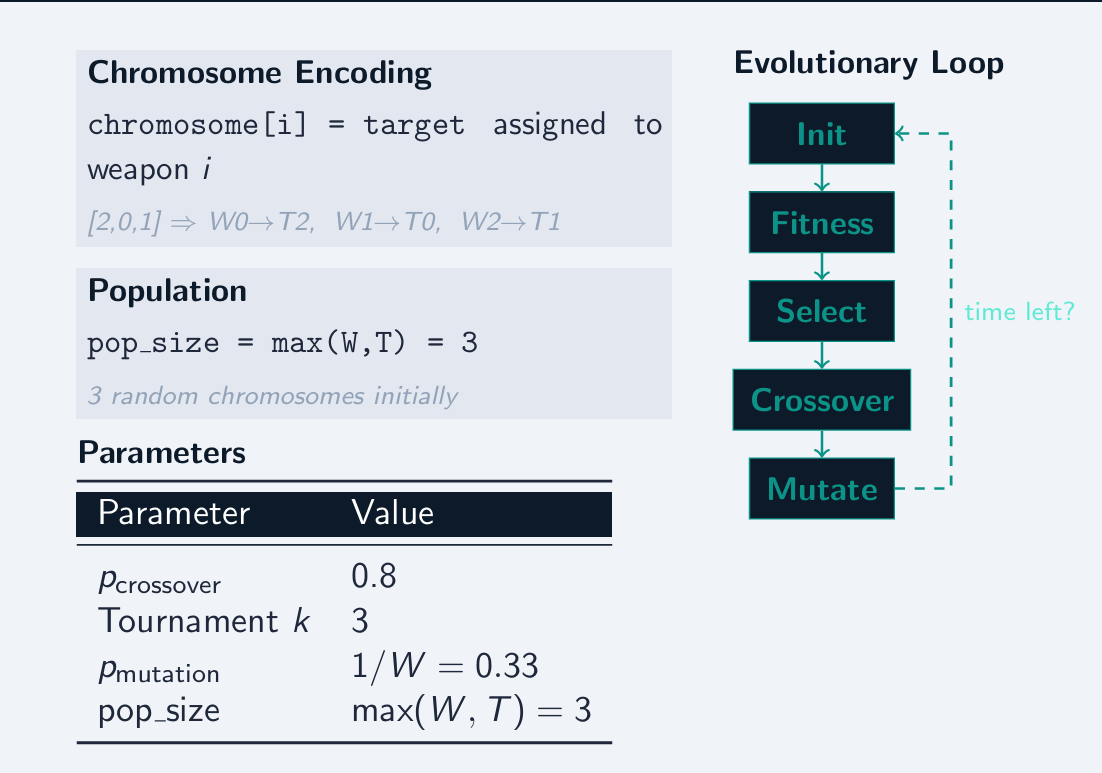
\includegraphics[width=\textwidth, height=0.85\textheight, keepaspectratio]{Screenshot 2026-03-29 165838.png}
    \end{column}
    % Right narrow column: text
    \begin{column}{0.32\textwidth}
      \vspace{1cm}

      Loop repeats until time budget exhausted.\\[6pt]
      Best solution is tracked across all generations.
    \end{column}
  \end{columns}
\end{frame}


% ─── SLIDE 6b: GA Pseudocode ─────────────────────────────────────────────────
\begin{frame}{Genetic Algorithm --- Pseudocode}

  \begin{columns}[T]
    % Left column: first image (pseudocode)
    \begin{column}{0.50\textwidth}
      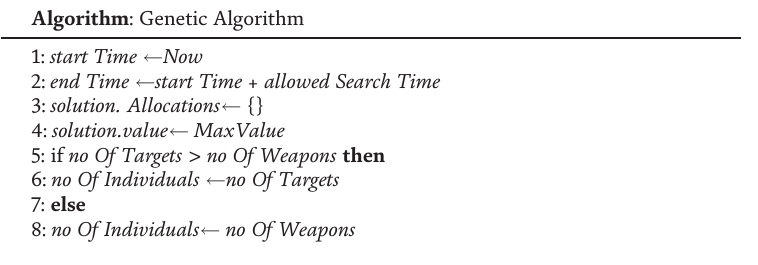
\includegraphics[width=\textwidth, height=0.85\textheight, keepaspectratio]{Screenshot 2026-03-29 170144.png}
    \end{column}

    % Right column: second image (flowchart/structure)
    \begin{column}{0.48\textwidth}
      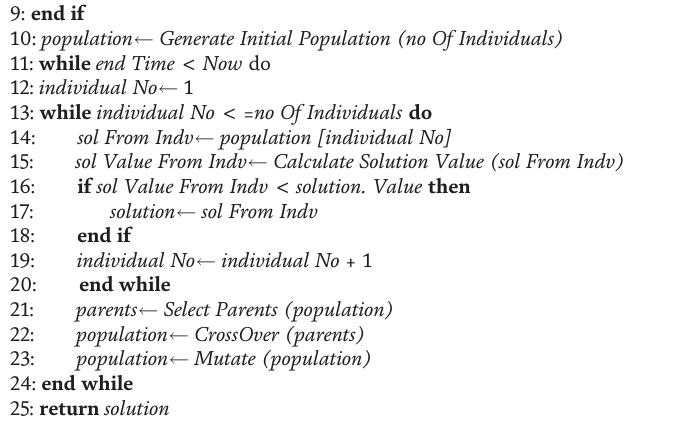
\includegraphics[width=\textwidth, height=0.85\textheight, keepaspectratio]{Screenshot 2026-03-29 170153.png}
    \end{column}
  \end{columns}

\end{frame}

% ─── SLIDE 7: GA Init & Fitness ───────────────────────────────────────────────
\begin{frame}{GA --- Step 1: Initialise Population \& Evaluate Fitness}
  \begin{columns}[T]
    \begin{column}{0.42\textwidth}
      \colorbox{navymid}{\color{teallt}\bfseries\small
        Random Population (pop\_size=3)}
      \vspace{3pt}

      \colorbox{offwhite}{\begin{minipage}{\linewidth}
        {\small\bfseries\color{navy} Ind 0:} {\small [2,0,1]}\\
        {\scriptsize\color{mygray} W0$\to$T2,\;W1$\to$T0,\;W2$\to$T1}
      \end{minipage}}
      \vspace{2pt}

      \colorbox{offwhite}{\begin{minipage}{\linewidth}
        {\small\bfseries\color{navy} Ind 1:} {\small [0,0,2]}\\
        {\scriptsize\color{mygray} W0$\to$T0,\;W1$\to$T0,\;W2$\to$T2}
      \end{minipage}}
      \vspace{2pt}

      \colorbox{offwhite}{\begin{minipage}{\linewidth}
        {\small\bfseries\color{navy} Ind 2:} {\small [1,2,0]}\\
        {\scriptsize\color{mygray} W0$\to$T1,\;W1$\to$T2,\;W2$\to$T0}
      \end{minipage}}
    \end{column}

    \begin{column}{0.54\textwidth}
      \colorbox{navymid}{\color{teallt}\bfseries\small
        Fitness for Ind 1: [0,0,2]}
      \vspace{4pt}

      {\small
      \begin{align*}
        \text{W0}\!\to\!\text{T0}:&\;
          \text{surv}[0] \mathrel{\times}= (1-0.3) = 0.7\\
        \text{W1}\!\to\!\text{T0}:&\;
          \text{surv}[0] \mathrel{\times}= (1-0.1) = 0.63\\
        \text{W2}\!\to\!\text{T2}:&\;
          \text{surv}[2] \mathrel{\times}= (1-0.5) = 0.5
      \end{align*}}

      {\small surv $= [0.63,\;1.0,\;0.5]$}\\[4pt]
      {\small $f = 10{\times}0.63 + 20{\times}1.0 + 30{\times}0.5
        = \mathbf{41.3}$}

      \vspace{0.3cm}
      \begin{tabular}{ccc}
        \toprule
        \rowcolor{navy}
          \color{white}\bfseries Ind &
          \color{white}\bfseries Chrom &
          \color{white}\bfseries Fit \\
        \midrule
        0 & [2,0,1] & 50.0 \\
        \rowcolor{lightgreen}
        \bfseries 1 & \bfseries[0,0,2] &
          \cellcolor{mygreen}\color{white}\bfseries 41.3$\star$ \\
        2 & [1,2,0] & 48.0 \\
        \bottomrule
      \end{tabular}
    \end{column}
  \end{columns}
\end{frame}

% ─── SLIDE 8: GA Selection + Crossover + Mutation ────────────────────────────
\begin{frame}{GA --- Step 2: Selection + Crossover + Mutation}
  \begin{columns}[T]
    \begin{column}{0.43\textwidth}
      \colorbox{navymid}{\color{teallt}\bfseries\small
        Tournament Selection (k=3)}
      \vspace{3pt}

      {\scriptsize Pick 3 random individuals $\to$ lowest fitness wins}\\[3pt]

      \begin{tabular}{ccc}
        \toprule
        \rowcolor{navy}
          \color{white}\bfseries Idx &
          \color{white}\bfseries Chrom &
          \color{white}\bfseries Fit \\
        \midrule
        0 & [2,0,1] & 50.0 \\
        \rowcolor{lightgreen}
        \bfseries 1$\star$ & \bfseries[0,0,2] &
          \cellcolor{mygreen}\color{white}\bfseries 41.3 \\
        2 & [1,2,0] & 48.0 \\
        \bottomrule
      \end{tabular}

      \vspace{4pt}
      {\small\bfseries\color{navy} P1 = P2 = [0,\,0,\,2]}
    \end{column}

    \begin{column}{0.53\textwidth}
      \colorbox{navymid}{\color{teallt}\bfseries\small
        Uniform Crossover ($p_c=0.8$)}
      \vspace{3pt}

      \begin{tabular}{lcccc}
        \toprule
        \rowcolor{navy}
          \color{white} &
          \color{white}g-0 & \color{white}g-1 & \color{white}g-2 \\
        \midrule
        \cellcolor{teal}\color{white}\bfseries P1 & 0 & 0 & 2 \\
        \cellcolor{teal}\color{white}\bfseries P2 & 0 & 0 & 2 \\
        \cellcolor{navymid}\color{teallt}\bfseries mask & T & F & T \\
        \cellcolor{lightgreen}\bfseries C1 & 0 & 0 & 2 \\
        \bottomrule
      \end{tabular}
    \end{column}
  \end{columns}

  \vspace{0.2cm}
  \colorbox{navymid}{\color{teallt}\bfseries\small
    Mutation ($p_m=1/3\approx0.33$) on C1=[0,0,2]}
  \vspace{3pt}

  \begin{tabular}{ccccc}
    \toprule
    \rowcolor{navy}
      \color{white}\bfseries Gene &
      \color{white}\bfseries rng.random() &
      \color{white}\bfseries $<0.33$? &
      \color{white}\bfseries Action &
      \color{white}\bfseries Result \\
    \midrule
    0 (W0) & 0.71 & No  & keep & 0 \\
    \rowcolor{lightyellow}
    \bfseries 1 (W1) & 0.12 &
      \cellcolor{amber}\color{white}\bfseries Yes &
      new random target &
      \cellcolor{amber}\color{white}\bfseries 2 \\
    2 (W2) & 0.55 & No  & keep & 2 \\
    \bottomrule
  \end{tabular}

  \vspace{3pt}
  {\small\bfseries\color{teal} Mutated C1 = [0,\,2,\,2]}
\end{frame}

% ─── SLIDE 9: GA Offspring Fitness ────────────────────────────────────────────
\begin{frame}{GA --- Step 3: Evaluate Offspring \& Update Best}
  {\bfseries\color{navy} After mutation, C1 = [0,\,2,\,2]}\\
  \sectionbar

  \begin{columns}[T]
    \begin{column}{0.52\textwidth}
      \colorbox{navymid}{\color{teallt}\bfseries\small
        Fitness for [0,\,2,\,2]}
      \vspace{4pt}

      {\small
      \begin{align*}
        \text{W0}\!\to\!\text{T0}:&\;
          \text{surv}[0] \mathrel{\times}= (1-0.3) = 0.7 \\
        \text{W1}\!\to\!\text{T2}:&\;
          \text{surv}[2] \mathrel{\times}= (1-0.2) = 0.8 \\
        \text{W2}\!\to\!\text{T2}:&\;
          \text{surv}[2] \mathrel{\times}= (1-0.5) = 0.4
      \end{align*}}

      {\small surv $= [0.7,\;1.0,\;0.4]$}\\[4pt]
      {\small $f = 10{\times}0.7 + 20{\times}1.0 + 30{\times}0.4
        = 7.0+20.0+12.0 = \mathbf{39.0}$}
    \end{column}

    \begin{column}{0.44\textwidth}
      \colorbox{navy}{\begin{minipage}{\linewidth}
        \vspace{0.2cm}\centering
        {\color{teal}\bfseries Best Update}\\[0.15cm]
        \colorbox{navymid}{\begin{minipage}{0.9\linewidth}\centering
          {\color{mygray}\small Before}\\
          {\color{white}\bfseries best = 41.3}
        \end{minipage}}\\[0.15cm]
        {\color{amber}\bfseries $39.0 < 41.3$ \checkmark}\\[0.15cm]
        \colorbox{teal}{\begin{minipage}{0.9\linewidth}\centering
          {\color{white}\small New Best!}\\
          {\color{white}\bfseries [0,2,2] $\to$ 39.0}
        \end{minipage}}
        \vspace{0.2cm}
      \end{minipage}}
    \end{column}
  \end{columns}

  \vspace{0.25cm}
  \colorbox{navymid}{\begin{minipage}{\linewidth}
    {\color{teallt}\small\itshape
     Loop continues --- new population replaces old;
     \texttt{best\_alloc} tracks the global best across all generations.}
  \end{minipage}}
\end{frame}

% ─── SLIDE 10: GA Final Result ────────────────────────────────────────────────
\begin{frame}{GA --- Final Result After All Generations}
  {\small\bfseries\color{navy} Best allocation found by GA:}\\[6pt]

  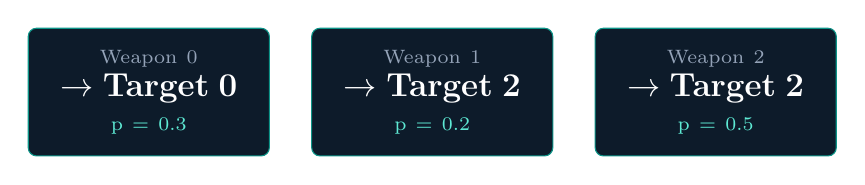
\begin{tikzpicture}
    \foreach \w/\t/\p [count=\i] in {0/0/0.3,1/2/0.2,2/2/0.5}{
      \node[fill=navy, draw=teal, rounded corners=3pt,
            inner sep=8pt, text width=2.5cm, align=center]
        at (\i*3.6cm-1.8cm, 0){
          {\color{mygray}\scriptsize Weapon \w}\\
          {\color{white}\large\bfseries $\to$ Target \t}\\
          {\color{teallt}\scriptsize p = \p}};
    }
  \end{tikzpicture}

  \vspace{0.2cm}
  \colorbox{amber}{\color{white}\bfseries\small
    allocation = [0,\; 2,\; 2]}

  \vspace{0.3cm}
  \colorbox{navymid}{\color{teallt}\bfseries\small Final Fitness Breakdown}
  \vspace{3pt}

  \begin{tabular}{lccc}
    \toprule
    \rowcolor{navy}
      \color{white}\bfseries Target &
      \color{white}\bfseries Value &
      \color{white}\bfseries Survival &
      \color{white}\bfseries Contribution \\
    \midrule
    Target 0 & 10 & 0.7 & $10\times0.7 = 7.0$ \\
    Target 1 & 20 & 1.0 & $20\times1.0 = 20.0$ \\
    Target 2 & 30 & 0.4 & $30\times0.4 = 12.0$ \\
    \midrule
    \rowcolor{teal}
      \color{white}\bfseries Total & & &
      \color{white}\bfseries $7.0+20.0+12.0 = 39.0$ \\
    \bottomrule
  \end{tabular}
\end{frame}

% ─── SLIDE 11: Comparison ─────────────────────────────────────────────────────
\begin{frame}{MMR vs GA --- Side-by-Side Comparison}
  \begin{tabular}{>{\columncolor{navymid}\color{teallt}\bfseries}l
                  >{\columncolor{offwhite}}p{3.9cm}
                  >{\columncolor{offwhite}}p{3.9cm}}
    \toprule
    \rowcolor{navy}
      & \multicolumn{1}{c}{\color{white}\bfseries MMR}
      & \multicolumn{1}{c}{\color{white}\bfseries Genetic Algorithm} \\
    \midrule
    Approach
      & Greedy --- one best step at a time
      & Evolutionary --- population-based search \\[3pt]
    Speed
      & Very fast $O(W^2\!\times\! T)$
      & Slower --- time-budget driven \\[3pt]
    Optimality
      & Local optimum only
      & Closer to global optimum \\[3pt]
    Allocation
      & [0,\;1,\;2]
      & [0,\;2,\;2] \\[3pt]
    Fitness
      & (compute via formula)
      & \bfseries 39.0 \\[3pt]
    Randomness
      & Deterministic
      & Stochastic (seed-based) \\
    \bottomrule
  \end{tabular}

  \vspace{0.25cm}
  \colorbox{navymid}{\begin{minipage}{\linewidth}
    {\color{teallt}\small\itshape
     GA finds a better solution (39.0) by exploring many chromosomes.
     MMR is faster but commits to early greedy choices.}
  \end{minipage}}
\end{frame}

% % ─── SLIDE 12: Key Takeaways ──────────────────────────────────────────────────
% \begin{frame}[plain]
%   \begin{tikzpicture}[remember picture, overlay]
%     \fill[navy] (current page.south west) rectangle (current page.north east);
%     \fill[teal] (current page.south west)
%       rectangle ([xshift=0.18cm] current page.north west);
%   \end{tikzpicture}

%   \vspace{0.4cm}
%   {\color{white}\large\bfseries Key Takeaways}\\
%   {\color{teal}\rule{6cm}{0.4pt}}\\[0.3cm]

%   \begin{enumerate}\itemsep9pt
%     \item {\color{teallt}\bfseries MMR is deterministic \& fast} ---
%       {\color{white}\small Greedy scan; assigns best pair each round.
%        No randomness, no iteration.}

%     \item {\color{teallt}\bfseries GA explores broadly} ---
%       {\color{white}\small Maintains a population; crossover \&
%        mutation discover better allocations over time.}

%     \item {\color{teallt}\bfseries GA found better result} ---
%       {\color{white}\small Fitness 39.0; evolutionary search avoids
%        early commitment to suboptimal choices.}

%     \item {\color{teallt}\bfseries Trade-off: speed vs quality} ---
%       {\color{white}\small MMR for real-time decisions.
%        GA when computation time allows a better solution.}
%   \end{enumerate}

%   \vspace{0.4cm}
%   \colorbox{navymid}{\begin{minipage}{0.95\linewidth}
%     {\color{mygray}\small
%      Instance: 3 Weapons $\times$ 3 Targets \;|\;
%      GA Best: [0,2,2] = 39.0 \;|\; MMR: [0,1,2]}
%   \end{minipage}}
% \end{frame}

\end{document}